% -*- TeX:Soft -*-
\documentclass[11pt]{article}
\usepackage{amsmath}
\usepackage{graphicx}
\usepackage{amsfonts}
\usepackage{listings}
\usepackage{optprog}
\usepackage{color}
\usepackage{makeidx}
\usepackage{epstopdf}
\usepackage[latin9]{inputenc}
\usepackage{moresize}
\usepackage{color}

\usepackage{xspace}
\usepackage{flafter}% Causes floats to show AFTER cited
\usepackage{hyperref} %clean files .aux, .toc, etc before using hyperref.

\definecolor{darkgreen}{rgb}{0.00,0.50,0.25}

\title{jMDP User's Guide}
\author{  Germ\'an Ria\~no, Andr\'es Sarmiento and Daniel F. Silva}
\date{}

\newcommand {\cA}{\ensuremath \mathcal{A}}
\newcommand {\cS}{\ensuremath \mathcal{S}}
\newcommand {\lil}{\lstinline}
\DeclareMathOperator*{\argmin}{argmin}
\newtheorem{rem}{Remark}

%\lstset{
  %basicstyle=\small,
  %language=java,
  %frame=single,
  %tabsize=2,
  %showstringspaces=false,
  %morecomment=[s][\color{darkgreen}]{/*}{*/},
  %morecomment=[l][\color{darkgreen}]{//},
  %morecomment=[s][\color{blue}]{/**}{*/},
  %morestring=[d][\color{blue}]{"}
%}

\definecolor{purple}{rgb}{0.40,0.00,0.45}
\definecolor{green}{rgb}{0.00,0.25,0.00}
\lstset{
    basicstyle=\ssmall,
    language=java,
    frame=single,
    keywordstyle=\color{purple}\bfseries,
    morestring=[d][\color{blue}]{"},
    numbers=left,
  	firstnumber=1,
  	numberfirstline=true,
}



%\textcolor[rgb]{0.00,0.50,0.25}{}
\newcommand{\lstinclude}[1]{
  %\lstset{title={\Large{File #1}},basicstyle=\small}
  %\lstinputlisting{../../../src/examples/jmdp/#1}
	\lstinputlisting{examples/#1}
}

\newcommand{\codeln}[1]{\lstinline[basicstyle=\normalsize\ttfamily, mathescape=true]|#1|}

\newcommand{\jMDP}{\codeln{jMDP}\xspace}
\newcommand{\mA}{\mathcal{A}}
\newcommand{\mS}{\mathcal{S}}
\DeclareMathOperator{\E}{\mathbb E}


%\lstset{language=[AspectJ]Java, basicstyle=\small,
%commentstyle=\footnotesize,
%tabsize=2,frame=single, breakautoindent=true}

\setlength{\oddsidemargin}{0pt} \setlength{\textwidth}{6.5in}
\setlength{\marginparsep}{0pt} \addtolength{\voffset}{-.8in}
\addtolength{\textheight}{1.5in}
\makeindex

\begin{document}
%\renewcommand{\includegraphics}[2][]{\framebox{File #2.eps Missing!}}

\maketitle
\tableofcontents

\section*{Introduction}

Java package for Markov Decision Process Package (JMDP) is an object oriented framework designed to model dynamic programming problems (DP) and Markov Decision Processes (MDPs).

\section{Java and Object Oriented Programming}


Java is a publicly available language developed by Sun
Microsystems. The main characteristics that Sun intended to have in Java
are:
\begin{itemize}
  \item Object-Oriented.
  \item Robust.
  \item Secure.
  \item Architecture Neutral
  \item Portable
  \item High Performance
  \item Interpreted
  \item Threaded
  \item Dynamic
\end{itemize}

Object Oriented Programming \index{Object Oriented Programming} (OOP)\index{OOP} is not a new idea. However it has not
have an increased development until recently. OOP is based on four key
principles:
\begin{itemize}
  \item abstraction.
  \item encapsulation
  \item inheritance
  \item polymorphism
\end{itemize}

An excellent explanation of OOP and the Java programming language can be
found in ~\cite{ld:jj}.

The abstraction capability is the one that interests us most. Java allows us to define abstract types like Actions, States, etc. We also define abstract functions like \lstinline!immediateCost()!.  We can program the algorithm in terms of this abstract objects and functions, creating a flexible tool. This tool can be used to define and solve DP problems. All the user has to do is to \textit{implement} the abstract functions. What it is particularly nice is that if a function is declared as abstract, then the compiler itself will require the user to implement it before attempting to run the
model.

\section{Markov Decision Process - The Mathematical Model}

The general problems that can be modeled and solved with the present framework can be classified in finite or infinite horizon problems. In any of these cases, the problem can be deterministic or stochastic. See Figure \ref{fig:classification}.

\begin{figure}[htb]  \centering
   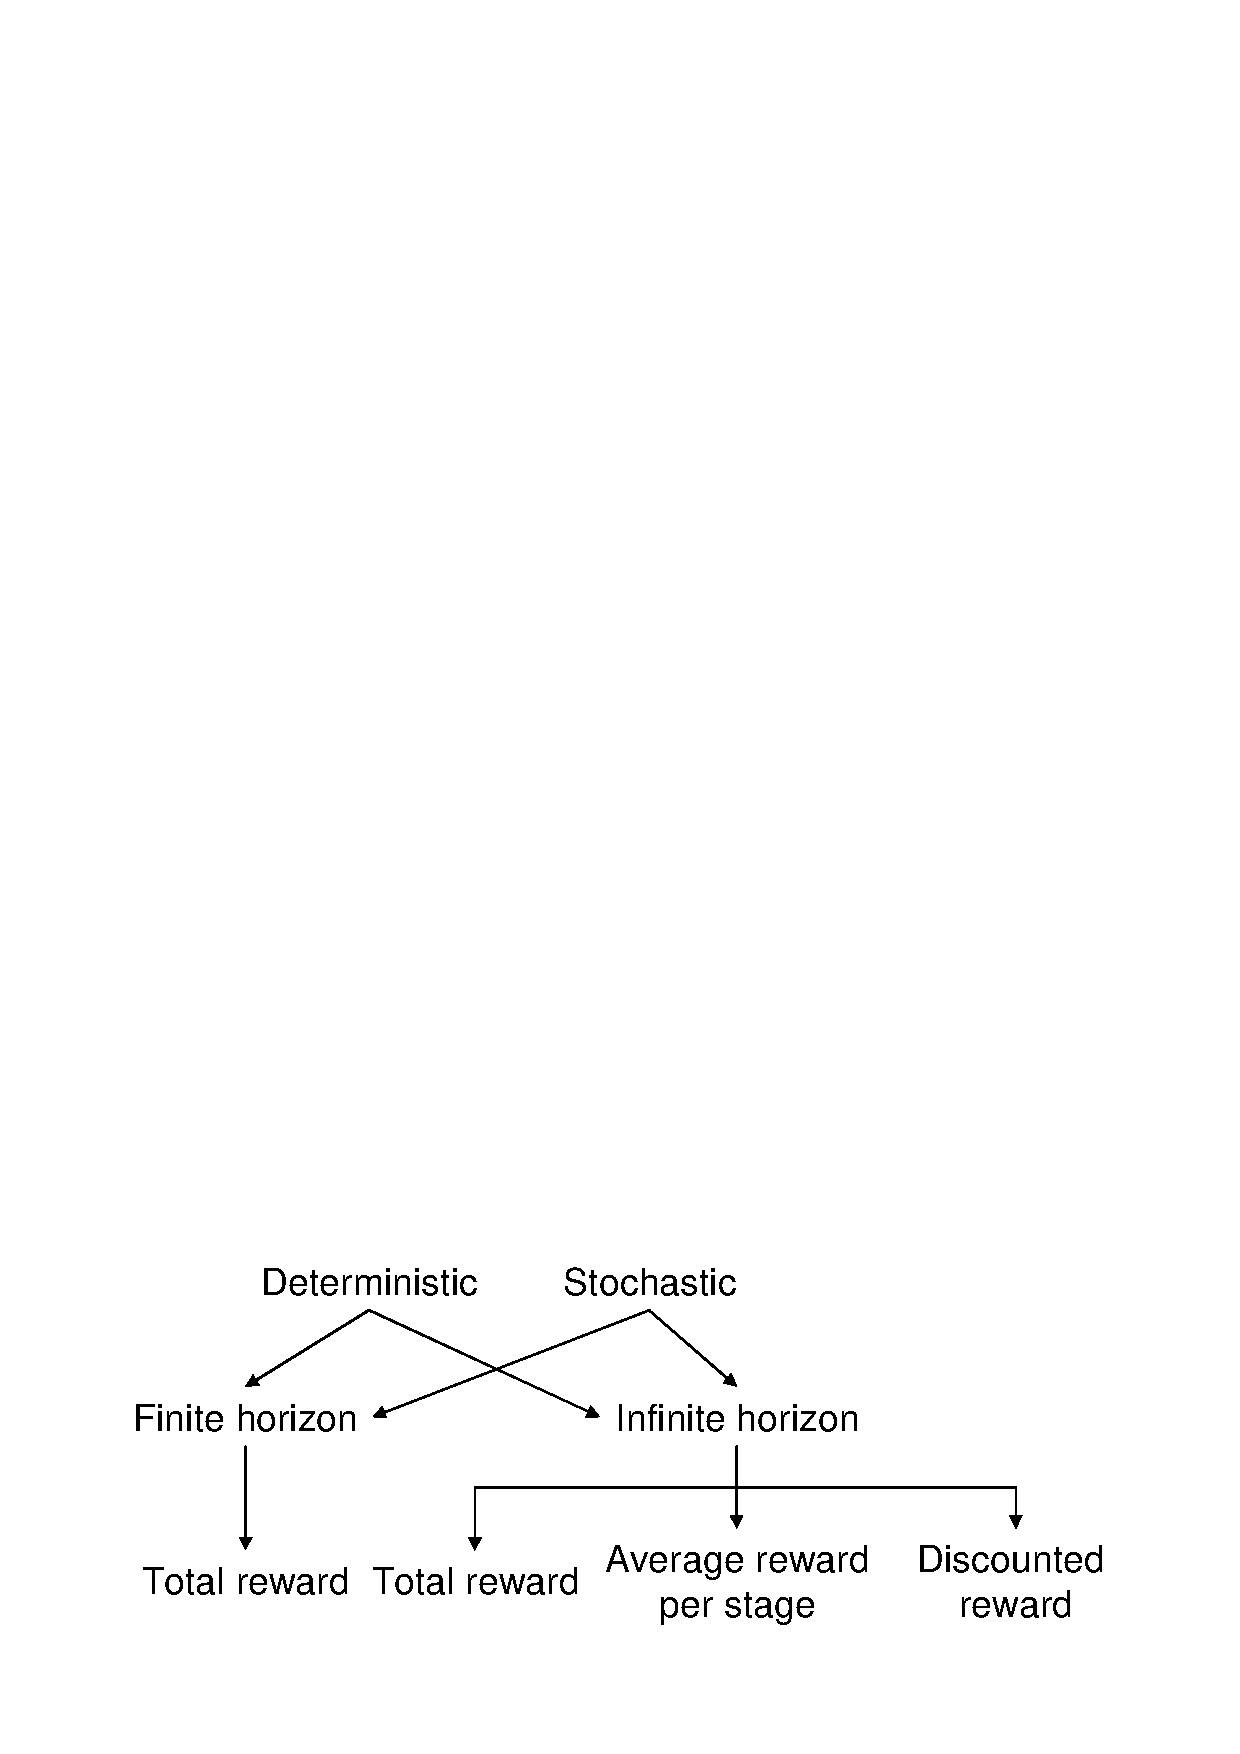
\includegraphics[width=4in]{taxonomy3}
    \caption{Taxonomy for MDP problems. WARNNING: ``rewards'' need to be changed to ``costs''.}
   \label{fig:classification}
\end{figure}

The deterministic problems are known as Dynamic Programming \index{Dynamic Programming} problems, and the stochastic problems are commonly called MDPs.

\subsection{Finite Horizon Problems}\index{Finite Horizon Problems}

We will show how a Markov Decision Process \index{Markov Decision Process} is built. Consider a discrete space, discrete time, bivariate random process $\{(X_t,A_t), t =0,1,\ldots,T \}$. Each of the $X_t \in \cS_t$ represents the state of the system at stage $t$, and each $A_t \in \cA_t$ is the action taken at that stage. The quantity $T<\infty$ is called the \emph{horizon}\index{horizon} of the problem.
The sets $\cS_t$ and $\cA_t$ are called the space state\index{space state} and the action space\index{action space},
respectively, and represent the states and actions available at stage $t$; we will assume that both are finite. The dynamics of the system are defined by two elements.
First, we assume the system has the  following Markov property
\begin{align*}
  P\{X_{t+1} =j|X_t &=i, A_t =a\} \\
& =  P\{X_{t+1} =j|X_t =i, A_t =a, X_{t-1} = i_{t-1}, A_{t-1} = a_{t-1} , \ldots,X_0=i_0\}.
\end{align*}
We call $p_{ijt}(a) = P\{X_{t+1} =j|X_t =i, A_t =a\}$ the \emph{transition probabilities}\index{Transition Probabilities}. Next, actions\index{action} are taken when a state is realized.
In general the action taken depends on the \emph{history} \index{history} of the process up to time $t$, i.e. $H_t = (X_0,A_0,X_1,A_1,\ldots,X_{t-1},A_{t-1},X_t)$.
A \emph{decision rule}\index{decision rule} is a function $\pi_t$ that given a history realization assign a probability distributions over the set $\cA$.  A sequence of decision rules $\pi = (\pi_0, \pi_1,\ldots, \pi_T)$ is called a \emph{policy}\index{policy}. We call $\Pi$ is the set of all policies. A policy is called Markov\index{Markov policy} if given $X_t$ all previous history becomes irrelevant, that is
\[P_\pi\{A_t=a|X_t=i,A_{t-1}=a_{t-1},X_{t-1}=i_{t-1},\ldots\} = P_\pi\{A_t=a|X_t=i\},\]
where we use $P_\pi\{\cdot\}$ to denote the probability measure (on events defined by ($X_t,A_t$)) induced by $\pi$. A Markov policy is called \emph{stationary}\index{stationary policy} if for all $t=0,1,\ldots$, and all $i\in\cS$ and $a \in \cA$,
\[P_\pi\{A_t=a|X_t=i\}=P_\pi\{A_0=a|X_0=i\}.\]

Notice that a stationary policy is completely determined by a single decision rule, and we have $\pi=(\pi_0,\pi_0,\pi_0,\ldots)$. A Markov policy is called \emph{deterministic}\index{deterministic policy} if there is a function $f_t(i)\in\cA$ such that
\[  P\{A_t=a|X_t=i\}=
\begin{cases}
  1 & \text{if } a=f_t(i)\\
  0 & \text{otherwise.}
\end{cases}\]
Whenever action $a$ taken from state $i$ at stage $t$, a finite cost $c_t(i,a)$\index{cost} is incurred. 
Consequently it is possible to define a total expected cost \index{total expected cost} $v_t^{\pi}(i)$ obtained from time $t$ to the final stage $T$ following policy $\pi$; this is called the \emph{value function}\index{value function}
\begin{equation}
v_t^{\pi}(i)=E_{\pi}\Bigg[\sum_{s=t}^T c_s(X_s,A_s)\Big|X_t=i\Bigg],\quad i\in \cS_0
\label{eq:finite}
\end{equation}
where $E_{\pi}$ is the expectation operator following the probability distribution associated with policy $\pi$. The problem is to find the policy $\pi \in \Pi$,  that maximizes the objective function shown above.
\[v_t^*(i) = \inf_{\pi \in \Pi} v_t^\pi(i).\]
Such optimal value function can be shown to satisfy \emph{Bellman's optimality equation}\index{Bellman's optimality equation}
\begin{equation}\label{eq:bellmanFinite}
  v_t^*(i) = \min_{a \in \mathcal{A}_t(i)} \Bigg \{ c_t(i,a) + \sum_{j \in \mathcal{S}_t(i,a)} p_{ijt}(a)v^*_{t+1}(j) \Bigg \} ,\quad i \in \mathcal{S},\, t=0,1,\ldots,T-1.
\end{equation}
where $\mathcal{A}_t(i)$ is the set of \emph{feasible actions}\index{feasible actions} that can be taken from state $i$ at stage $t$ and $\mathcal{S}_t(i,a)$ is the set of reachable states from state $i$ taking action $a$ at stage $t$. Observe that equation (\ref{eq:bellmanFinite}) implies an algorithm to solve the optimal value function, and consequently the optimal policy. It starts from some final values of $v_T(i)$ and solves backward the optimal decisions for the other stages. Since the action space $\cA_t$ is finite, the Bellman equation shows that it is possible to find a deterministic decision rule $f_t(i)$ (and hence a deterministic policy) that is optimal, by choosing in every stage in every state the action that maximizes the right hand side (breaking ties arbitrarily).


\subsection{Infinite Horizon Problems}\index{Infinite Horizon Problems}

Consider a discrete space discrete time bivariate random process $\{(X_t,A_t), t \in \mathbb{N} \}$. Notice the time horizon is now infinite. Solving a general problem like this is difficult unless we make some assumptions about the regularity of the system. In particular we will assume that the the system is  \emph{time homogeneous}, this means that at every stage the space state and action space remain constant and  the transition probabilities are independent of time $p_{ijt}(a)= p_{ij}(a) = P\{X_{t+1}=j| X_t=i,A_t=a\}$ for all $t=0,1,\ldots$. Costs are also time homogeneous so $c_t(i,a)=c(i,a)$ stands for the cost incurred when action $a$ is taken from state $i$. However, it is customary to define two objective functions, besides total cost: discounted cost, and average cost. We will explain these three problems in the next subsections.

\subsubsection{Discounted Cost}

In the discounted cost problem the costs in the first stages are more important than the later ones. In particular, a cost incurred at time $t$ is assumed to have a present value $\alpha^tr(i,a)$, where $0<\alpha<1$ is a discount factor. If the interest per period is $r$ then $\alpha=1/(1+r)$. The total expected discounted cost gives rise to a value function under policy $\pi$ defined as
\begin{equation}
v_{\alpha}^{\pi}(i)=E_{\pi}\Bigg[\sum_{t=0}^\infty \alpha^t c(X_t,A_t)\Big|X_0=i\Bigg],\quad i\in \cS
\label{eq:discounted}\end{equation}
 In this case, the optimal value function is

\[v_{\alpha}^*(i)=\inf_{\pi \in \Pi} v_{\alpha}^{\pi}(i),\]
and it can be shown that it satisfies the following Bellman's optimality equation \index{Bellman's optimality equation}
\begin{equation}\label{eq:bellmanDiscounted}
  v_{\alpha}^*(i) = \min_{a \in \mathcal{A}(i)} \Bigg \{ c(i,a) + \alpha\sum_{j \in \mathcal{S}(i,a)} p_{ij}(a)v_{\alpha}^*(j) \Bigg \} ,\quad i \in \cS,
\end{equation}
where $\cA(i)$ is the set of feasible actions from state $i$ in any stage and $\cS(i,a)$ is the set of reachable states. Notice that since $t$ does not appear in the equation it is possible to find an stationary policy that is optimal.

There are various algorithms for solving the discounted cost problem. One of them is almost implicit in equation (\ref{eq:bellmanDiscounted}). The algorithm is called \emph{Value Iteration} \index{Value Iteration algorithm} and begins with some initial values $v_{\alpha}^{(0)}(i)$ and iteratively defines the $n$-th iteration value function $v_{\alpha}^{(n)}(i)$ in terms of $v_{\alpha}^{(n-1)}(i)$ according to
\[  v_{\alpha}^{(n)}(i) = \min_{a \in \cA(i)} \Bigg \{ c(i,a) + \alpha\sum_{j \in \mathcal{S}(i,a)} p_{ij}(a)v_{\alpha}^{(n-1)}(j) \Bigg \} ,\quad i \in \mathcal{S}.
\]
It can be shown that for $0<\alpha<1$ the algorithm converges regardless of the initial function. For further details see Bertsekas\cite{bertsekas} or Stidham\cite{stidham}. If the algorithm has stopped after $N$ iterations , then the recommended policy will be
\[f(i) = \argmin_{a \in \mathcal{A}(i)} \Bigg \{ c(i,a) + \alpha\sum_{j \in \mathcal{S}(i,a)} p_{ij}(a)v_{\alpha}^{(N)}(j) \Bigg \} ,\quad i \in \cS.\]
A policy is said to be \emph{$\epsilon$-optimal}\index{$\epsilon$-optimal} if its corresponding value function satisfies $\max|v_\beta(i)-v^*(i)|<\epsilon$. If the previous algorithm stops when $\max|v_\alpha^{(n)}( i ) - v_\alpha^{ (n-1) }(i)|<\epsilon(1-\alpha)/(2\alpha))$ then it can be shown that the stationary policy $\pi=(f,f,\ldots)$ is $\epsilon$-optimal.

The \emph{Policy Iteration algorithm} \index{Policy Iteration algorithm} starts with a deterministic policy $f(i)$ and through a series of iterations find improving policies. In every iteration for a given policy $f(i)$ its corresponding value function  is computed solving the following linear system
\begin{equation}\label{eq:lin_system}
 v^f(i) = c(i,f(i)) + \alpha\sum_{j \in \mathcal{S}(i,f(i))} p_{ij}(f(i))v^{f}(j) ,\quad i \in \mathcal{S},
\end{equation}
where $v^f (i)$ if the total expected discounted cost under the deterministic stationary policy $\pi=\{f, f, f, \ldots\}$. A new policy $f'$ is found through the following policy-improvement step
\[f'(i) = \argmin_{a \in \mathcal{A}(i)} \Bigg \{ c(i,f(i)) + \alpha\sum_{j \in \mathcal{S}(i,a)} p_{ij}(f(i))v^f(j) \Bigg \} ,\quad i \in \mathcal{S}.\]
After a succession of value computation and policy improvement steps the algorithm stops when no further improvement can be obtained.
This guarantees an optimal solution instead of an $\epsilon$-optimal one, but can be very time consuming to solve the systems.
The discounted cost problem can also be solved with a linear program. See \cite{stidham} for details.

\subsubsection{Total Cost}

The value function in the total cost case is given by
\[v^{\pi}(i)=E_{\pi}\Bigg[\sum_{t=0}^\infty c(X_t,A_t)\Big|X_0=i\Bigg],\quad i\in \cS\]
and the optimal value function is
\[v^*(i)=\sup_{\pi \in \Pi} v^{\pi}(i)\]
The total cost problem can be thought of as a discounted cost with $\alpha=1$.
However, the algorithms presented do not work in this case. The policy evaluation in the policy iteration algorithm fails since the linear system \eqref{eq:lin_system} is always singular; and there is no guarantee that the value iteration algorithm  converges unless we impose some additional condition. This is due to the fact that the total cost might be infinite. One of the conditions is to assume that there exists an absorbing state with zero-cost and that every policy eventually reaches it. (Weaker conditions can also be used, see \cite{bertsekas} ). This problem is also called the Stochastic Shortest Path'index{Stochastic Shortest Path} problem, since since if  expected total cost can be thought of as the minimal expected cost accumulated before absorption in a graph with random costs.

\subsubsection{Average Cost}

In an ergodic chain that reaches stable state, the steady state probabilities are independent of the initial state of the system. Intuitively, the average cost per stage should be a constant regardless of the initial state. So the value function is

\[\overline{v}^{\pi}(i)=\lim_{T\rightarrow \infty}\frac{1}{T}E_{\pi}\Bigg[\sum_{t=0}^T c(X_t,A_t)\Big|X_0=i\Bigg],\quad i\in \cS\]
and the optimal value function is the same for every state

\[g=\overline{v}^*(i)=\inf_{\pi \in \Pi} \overline{v}^{\pi}(i)\]

The average cost per stage problem can be obtained by solving the following linear program
\begin{subequations}
  \begin{optprog}
    g = \optaction[x_{ia}]{min} & \objective{\sum_{i\in \cS}\sum_{a\in \cA(i)} c(i,a)x_{ia} }\label{eq:obj}\\
    s.t. & \sum_{a\in \cA(j)} 
      \sum_{\{i:j\in \cS(i,a)\}}p_{ij}(a)x_{ia} 
        &=& \sum_{a\in\cA(i)} x_{ja} & j\in \cS \label{eq:balance}\\
    and        &\sum_{i\in \cS}\sum_{a\in \cA(i)} x_{ia} & = & 1, \label{eq:normal}
  \end{optprog}
\end{subequations}
where the solution is interpreted as
\[x_{ia}=\lim_{t\rightarrow0}P\{X_t=i,A_t=a\} \qquad i\in\cS, a\in\cA(i).\]
The equation \eqref{eq:obj} is the average cost per transition in steady state, \eqref{eq:balance} are analogous to the balance equations in every markovian system and \eqref{eq:normal} is the normalization condition. The optimal policy can be obtained after the LP has been solved as
\[ \pi_i(a)= P\{A_t=a|X_t=i\} = \frac{x_{ia}}{\sum_{b\in\cA(i)} x_{ib}}. \qquad i\in\cS, a\in\cA(i)\]
It can be shown that for every $i\in\cS$ the is only one $a\in\cA(i)$ that is positive, so the optimal policy is always deterministic. There is also an iterative solution based on a modification of the value iteration algorithm. See \cite{mp:mdp} for details.

\begin{rem}
It may seem to the reader that the infinite horizon admits more type of cost functions that the finite counterpart. That is not the case. The fact that the cost function depends on $t$, allows us to define a discounted cost as $c_t(i,a)=\alpha^tc(i,a)$, and an average cost as $c_t(i,a)=\frac{1}{T}c(i,a)$.
\end{rem}


\subsection{Deterministic Dynamic Programming}

This is a particular case of the finite horizon problem defined earlier. When the set of reachable states $\mathcal{S}_t(i,a)$ has only one state for all $t \in \mathbb N, \, i \in \cS, \, a \in \cA$, then it is clear that all the probability of reaching this state has to be $1.0$, and $0$ for every other state. This would be a deterministic transition. So it is possible to define a transition function $h:\cS\times \cA \times \mathbb N \rightarrow \cS$, that assigns to each state and action to be taken at the given stage, a unique destination state. Under this conditions, the Bellman equation would look like
\[v_t(i) = \min_{a \in \mathcal{A}_t(i)} \Bigg \{ c_t(i,a) + v_{t+1}\big(h(i,a,t)\big) \Bigg \} ,\quad i \in \mathcal{S}, t\in \mathbb{N}.\]
Naturally, there are also infinite horizon counterparts as in the probabilistic case.


\subsection{Main modeling elements in MDP}

Recall the Bellman equation (\ref{eq:bellmanFinite}). As explained before, $X_t$ and $A_t$ are the state and the action taken at stage $t$ respectively. The set $\mathcal{A}_t(i)$ is the set of actions that can be taken from state $i$ at stage $t$. So the optimal action is selected only from this feasible action set, for the statement to make sense. In the equation, the first cost is taken, and then it is added to the expected future value function.

The expected future value function is a sum over the states in $\mathcal{S}_t(i,a)$. This is the set of reachable states from state $i$ given that action $a$ is taken at stage $t$. If this set was not defined, then the sum would be over all the possible states $\mathcal{S}$, and its value would be the same, only that there would be many probabilities equal to zero.

As a summary, if the elements in Table \ref{tb:elems} are clearly identified, then it is possible to say that the Markov Decision Process has been defined.

\begin{table}[ht]
  \centering
  \begin{tabular}{|l|c|}
    \hline
    \multicolumn{1}{|c|}{Element} &  \multicolumn{1}{|c|}{Mathematical} \\
    \multicolumn{1}{|c|}{} &  \multicolumn{1}{|c|}{representation} \\
    \hline
    \hline
      States & $X_t \in \mathcal{S}$ \\
      \hline
      Actions & $A_t \in \mathcal{A}$ \\
      \hline
      Feasible actions & $\mathcal{A}_t(i)$ \\
      \hline
      Reachable states & $\mathcal{S}_t(i,a)$ \\
      \hline
      Transition probabilities & $p_{ijt}(a)$ \\
      \hline
      Costs & $c_t(i,a)$ \\
      \hline
  \end{tabular}\caption{Main elements}\label{tb:elems}
\end{table}


\section{Framework Design}

As stated before, the intention is to make this framework as easy to use as possible. An analogy is stated between the mathematical elements presented above and the computational elements that will be explained. There is first a general overview of the framework, and specific details of each structure will be presented afterwards. This first part should be enough to understand the examples.

The framework is divided in two packages. The modeling package is called \lstinline!jmdp!, and the solving package is \lstinline!jmpd.solvers!. The user does not need to interact with this second one, because a standard solver is defined for every type of problem. However, as the user gains experience he mights want to fine-tune the solvers or even define his/her own solver by using the package \lil!jmdp.solvers!.

The following steps will show how to model a problem. An inventory problem will be used.

\begin{enumerate}
  \item \textbf{Defining the states}. The first thing to do when modeling a problem, is to define which will be the states. Each state $X_t$ is represented by an object or class, and the user must modify the attributes to satisfy the needs of each problem. The class \lstinline!State! is declared abstract and can not be used explicitly; the user must extend class \lstinline!State! and define his own state for each type of problem. Once each state has been defined, a set of states $\cS$ can be defined with the class \lstinline!States!. For example, in an inventory problem, the states are inventory levels. The following file defines such a class. It has a constructor, and, very important implemente \lil!compareTo()! to establish a total ordering among the states. If no comparator is provided, then the sorting will be made according to the name, which might be very inefficient in real problems.

\lstinclude{InvLevel.java}



\item \textbf{Defining the actions}.The next step is to define the actions of the problem. Again, each action $A_t$ is represented by an object called \lstinline!Action!, and this is an abstract class that must be extended in order to use it. In an inventory problem, the actions that can be taken from each state are orders placed. %A set of actions $\cA$ can be defined with class \lstinline!Actions!.

\lstinclude{Order.java}

\item \textbf{Defining the problem}. In some way, the states and actions are independent of the problem itself. The rest of the modeling corresponds to the problem's structure that is also represented by an object. In this case, the object is more complex than the ones defined earlier, but it combines the important aspects of the problem. The classes that represent the problem are also abstract classes and must be extended in order to be used. See table (\ref{tab:TypesOfProblems}) for reference on which class to extend for each type of problem.

\begin{table}[ht]
  \centering
    \begin{tabular}{|c|c|}
      \hline
      Type of Problem & Class to be extended\\
      \hline
      Finite Horizon Dynamic Programming Problem & \lstinline!FiniteDP<S,A>!\\
      Infinite Horizon Dynamic Programming Problem & \lstinline!InfiniteDP<S,A>!\footnote{Not implemented yet}\\
      Finite Horizon MDP & \lstinline!FiniteMDP<S,A>!\\
      Infinite Horizon MDP & \lstinline!InifiniteMDP<S,A>!\\
      \hline
    \end{tabular}
  \caption{Types of Problems}
  \label{tab:TypesOfProblems}
\end{table}

\lstset{title=,caption=}
\begin{lstlisting}
public class InventoryProblem extends FiniteMDP<InvLevel,Order>{

}
\end{lstlisting}

Once one of these classes is extended in a blank editor file, compilation errors will prompt up. This doesn't mean the user has done anything wrong, it is just a way to make sure all the requisites are fulfilled before solving the problem. Java has a feature called generics that allows safe type transitions. In the examples, whenever \lstinline!S! is used, it stands for \lstinline!S extends State! that is the class being used to represent a state. In the same way \lstinline!A! is the representation of \lstinline!A extends Action!. In the inventory example, class \lstinline!FiniteMDP<S,A>! will be extended and the editor will indicate the user that there are compilation errors because some methods have not yet been implemented. This means the user must implement this methods in order to model the problem, and also for the program to compile. It is necessary that the state and the action that were defined earlier are indicated in the field \lstinline!<S,A>! as state and action as shown in the example. This will allow the methods to know that this class is using these two as states and actions respectively.

\item \textbf{Feasible actions}. The first of these methods is \lstinline!public Actions getActions(S i, int t)!. For a given state $i$ this method must return the set of feasible actions $\cA(i)$ that can be taken at stage $t$. Notice that the declaration of the method takes element \lstinline!i! as of type \lstinline!S! but in the concrete example, the compiler knows the states that are being used are called \lstinline!InvLevel! and so changes the type.

\begin{lstlisting}
public Actions getActions(InvLevel i, int t){
  Actions<Order> actionSet = new ActionsCollection<Order>();
  for(int n=0; n<=K-i.level; n++){
    actionSet.add(new Order(n));
  }
  return actionSet;
}
\end{lstlisting}

The example procedure returns the actions corresponding to the set $\{0,1,\ldots,K-i\}$, the user can declare an empty set called \lstinline!actionSet! of type \lstinline!ActionsCollection<Order>!, which is an easy-to-use extension of \lstinline!Actions<A>!. The generics use is indicating that the set will store objects of type \lstinline!Order!. Then for each iteration of the for cycle, create a new order and this new action is added to the set. After adding all the actions needed, the method returns the set of actions.

\item \textbf{Reachable states}. The second method in the class \lstinline!FiniteMDP<S,A>! that must be implemented \lstinline!public States reachable(S i, A a, int t)! indicates the set of reachable states $\cS_t(i,a)$ from state $i$ and given that action $a$ is taken at stage $t$ . The example shows how to define the set of states $\{0,1,\ldots,a+i\}$. First declare an empty set called \lstinline!statesSet! of type \lstinline!StatesCollection<InvLevel>! which is an easy-to-use extension of \lstinline!States<S>!, that indicates this set will store objects of type \lstinline!InvLevel!. Then a for cycle adds a state for each value between 0 and $a+i$.
\lstset{title=,caption=}
\begin{lstlisting}
public States reachable(InvLevel i, Order a) {
  States<InvLevel> statesSet = new StatesCollection<InvLevel>();
  for(int n=0;n<=a.size+i.level;n++)
    statesSet.add(new InvLevel(n));
  return statesSet;
}
\end{lstlisting}

\item \textbf{Transition Probabilities}. The method \lstinline!public double prob(S i, S j, A a)! is still pending to be implemented and represents the transition probabilities $p_{ijt}(a)$.

\item \textbf{Costs}. The final method is the one representing the cost $c_t(i,a)$ received by taking action $a$ from state $i$ represented by the method \lstinline!public double immediateCost(S i, A a)!. Once these methods are implemented the class should compile.

\item \textbf{The \lstinline!main! method}. In order to test the model and solve it, the class may also have a \lstinline!main! method. This is of course not necessary, since the class can be called from other classes or programs provided you have been careful to declare it constructor public. The following example shows that the name of the class extending \lstinline!FiniteMDP! is \lstinline!InventoryProblem! so the \lstinline!main! method must first declare an object of that type, with the necessary parameters determined in the constructor method. Then the \lstinline!solve()! method must be called from such and the problem will call a default solver, solve the problem, store the optimal solution internally. You can obtain information about the optimal policy and value functions by calling the \lil!getOptimalPolicy()! and \lil!getoptimalValue()! methods. There is also a convenience method called \lil!printSolution()! which prints the solution in standard output.


\begin{lstlisting}
public static void main(String args[]) {

InventoryProblem prob = new InventoryProblem(maxInventory,
  maxItemsPerOrder, truckCost, holdingCost, theta);

prob.solve()
prob.printSolution()
}
\end{lstlisting}
\end{enumerate}

\begin{figure}[htb]  \centering
  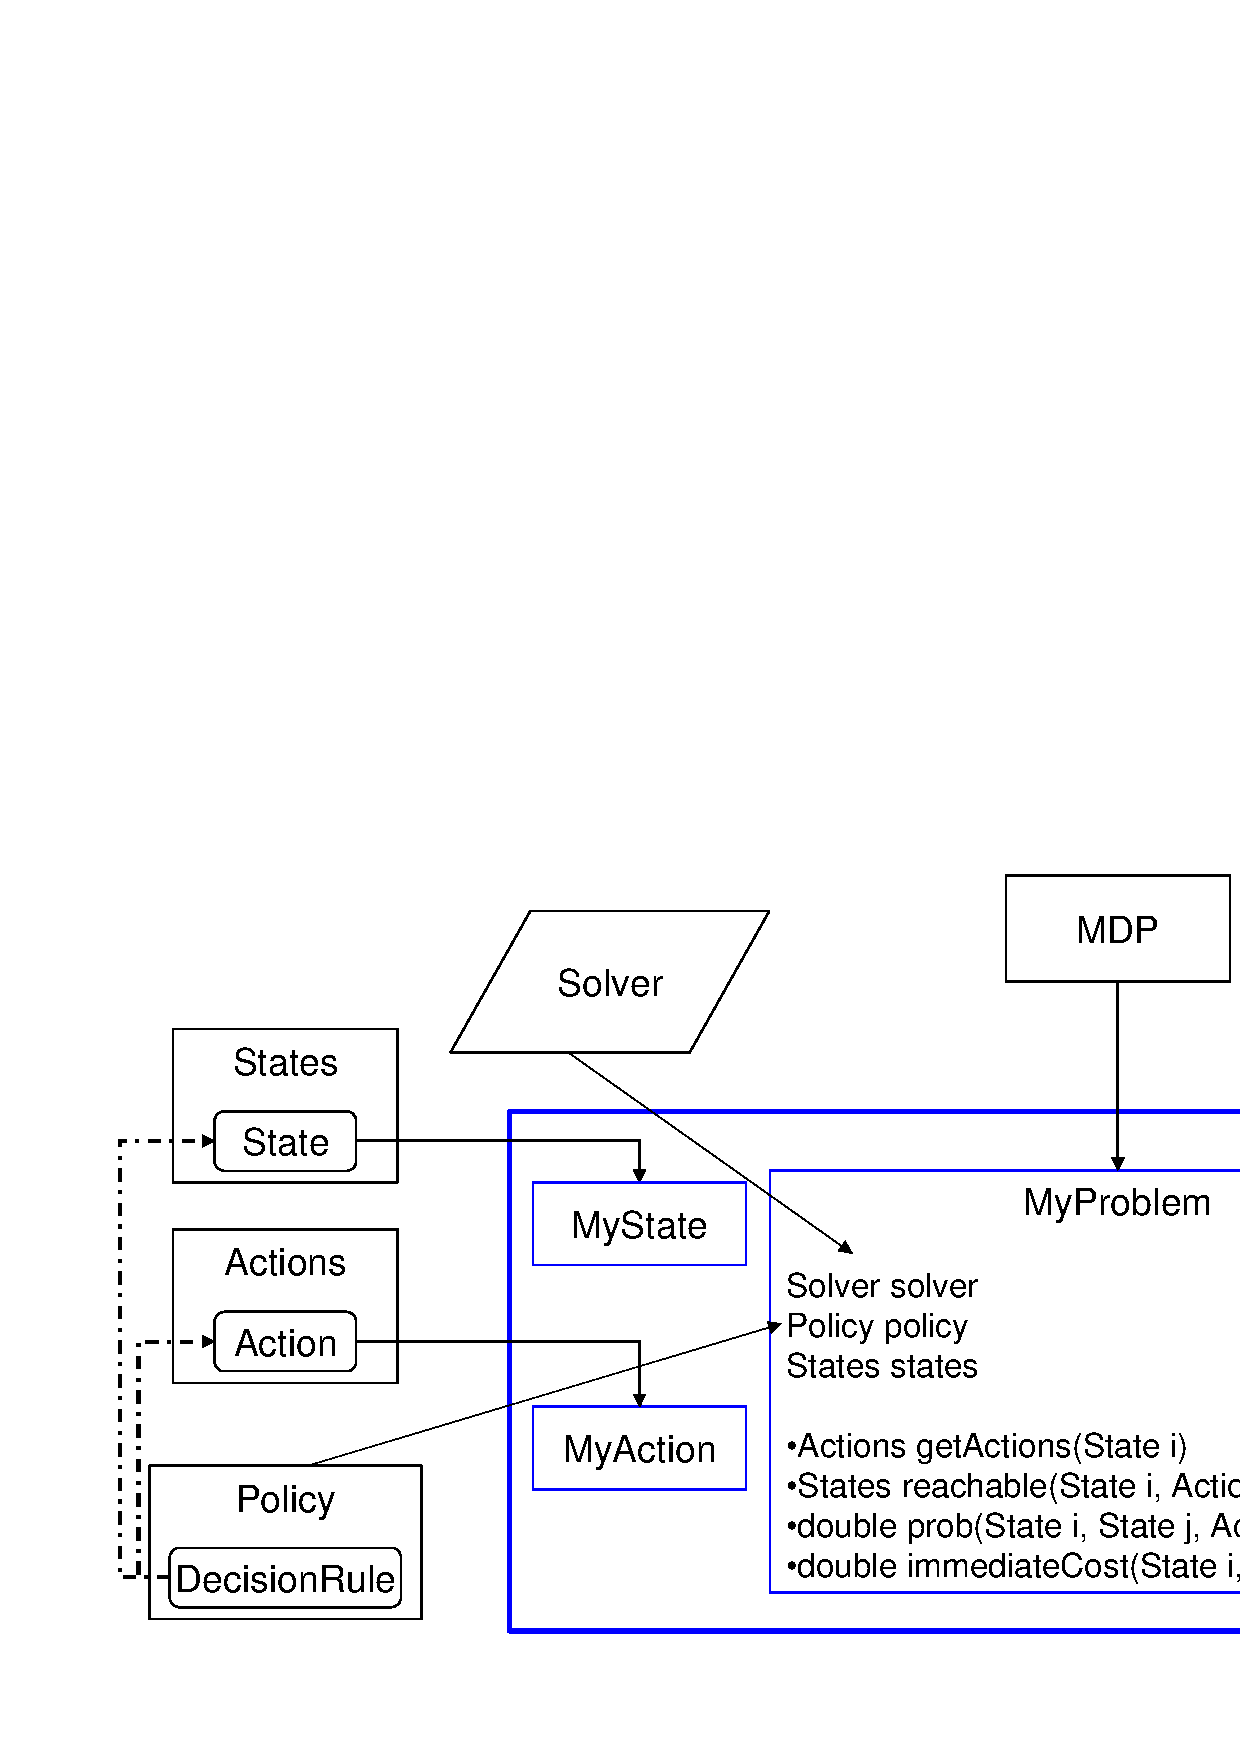
\includegraphics[height=2.7in]{ProblemStructure}%[height=2.7in]
  \caption{Problem's structure.}
\end{figure}

\begin{center}
  \begin{tabular}{|l|c|l|}
    \hline
    \multicolumn{1}{|c|}{Element} &  \multicolumn{1}{|c|}{Mathematical} & \multicolumn{1}{|c|}{Computational}\\
    \multicolumn{1}{|c|}{} &  \multicolumn{1}{|c|}{representation} & \multicolumn{1}{|c|}{representation}\\
    \hline
    \hline
      States & $X_t \in \mathcal{S}$ & \lstinline!public class MyState extends State!\\
      \hline
      Actions & $A_t \in \mathcal{A}$ & \lstinline!public class MyAction extends Action!\\
      \hline
      Process & $\{X_t,A_t\}$ & \lstinline!public class MyProblem extends FiniteMDP<S,A>!\\
      \hline
      Feasible actions & $\mathcal{A}_t(i)$ & \lstinline!public Actions getActions(S i, int t)!\\
      \hline
      Reachable states & $\mathcal{S}_t(i,a)$ & \lstinline!public States reachable(S i, A a, int t)!\\
      \hline
      Transition probabilities & $p_{ijt}(a)$ & \lstinline!public double prob(S i, S j, A a, int t)!\\
      \hline
      Costs & $c_t(i,a)$ & \lstinline!public double immediateCost(S i, A a, int t)!\\
      \hline
  \end{tabular}
\end{center}

For details on the construction of specifc sets, modifying the solver or solver options, see the Java documentation and the Advanced Features section.

\section{Examples}

This sections shows some problems and their solution with JMDP in order to illustrate its use. The examples cover the usage of the \lstinline!DP!, \lstinline!FiniteMDP!, and \lstinline!InfiniteMDP! classes.

\subsection{Deterministic inventory problem}

Consider a car dealer selling identical cars. All the orders to the distributor have to be placed on Friday eve and arrive on Monday morning before opening. The car dealer is open Monday to Friday. Each car is bought at USD \$20.000 and sold at USD\$22.000. A transporter charges a fixed fee of USD\$500 per truck for carrying the cars from the distributor to the car dealer, and each truck can carry 6 cars. The exhibit hall has space for 15 cars. If a customer orders a car and there are not cars available, the car dealer gives him the car a soon as it gets with a USD\$1000 discount. The car dealer does not allow more than 5 pending orders of this type. Holding inventory implies a cost of capital of 30\% annually. The marketing department has handed in the following demand forecasts, for the next 12 weeks, shown in table (\ref{tab:demands}).

\begin{table}[htb]  \centering
\begin{tabular}{|c|c|c|c|c|c|c|c|c|c|c|c|c|}
\hline
\multicolumn{1}{|c|}{} & \multicolumn{12}{|c|}{Weeks}\\
\hline
$t$&1&2&3&4&5&6&7&8&9&10&11&12\\
\hline
$D_t$&10& 4& 3& 6& 3& 2& 0& 1& 7& 3& 4& 5  \\
\hline
\end{tabular}
\caption{Demand forecast.}\label{tab:demands}
\end{table}

Let's first formulate the mathematical model, and then the computational one. The parameters in the word problem are in Table \ref{tab:parameters1}.

\begin{table}[ht]
\begin{center}
\begin{tabular}{ll}
$K$ & Fixed cost per truck.\\
$c$ & Unit cost.\\
$p$ & Unit price.\\
$D_t$ & Demand at week $t$.\\
$h$ & Holding cost per unit per week.\\
$b$ & Backorder cost.\\
$M$ & Maximum exhibit hall capacity.\\
$B$ & Maximum backorders allowed.\\
$L$ & Truck's capacity.\\
$T$ & Maximum weeks to model.
\end{tabular}
\caption[\textbf{Parameters:}]{Parameters}
\label{tab:parameters1}
\end{center}
\end{table}

The problem will be solved using dynamic programming to determine the appropriate amount to order in each week in order to minimize the costs. The problem has a finite horizon and is deterministic.

\begin{enumerate}
  \item States. Each state $X_t$ is the inventory level at each stage $t$, where the stages are the weeks. When there are backorders, they will be denoted as a negative inventory level. The set of states $\cS = \{-B, \ldots, 0, \ldots, M  \}$ are all the levels between the negative maximum backorders adn the maximum inventory level.
  \item Actions. Each action $A_t$ is the order placed in each stage $t$. The complete set of actions are the orders from 0 to the addition of the maximum exhibit hall's capacity and the maximum backorders allowed. $\cA = \{0,\ldots,B+M\}$.
  \item Feasible Actions. For each state $i$ the feasible actions that can be taken are those that will not exceed the exhibit hall's capacity. Ordering 0 is the minimum order and is feasible in every state. The maximum order feasible is $M-i$, so the feasible set of actions for each state $i$ is $\cA_t(i) =\{0,\ldots,M-i\}$.
  \item Destination. The destination state when action $a$ is taken from state $i$ is the sum of the cars in that state and the cars that are ordered, minus the cars that are sold. $h(i,a,t)=i+a-D_t$.
  \item Costs. Finally, the cost incured depends on various factors. The ordering cost is only charged when the order is positive, and charged per truck. The holding cost is charged only when there is positive stock, and the backorder cost charged only when there is negative stock. There is finally a profit for selling each car given by the difference between price and cost.

  \begin{equation*}
    OC(a)=      \left\lceil \frac{a}{L}\right\rceil  
  \end{equation*}

  \begin{equation*}HC(i)+BC(i)=\left\{
    \begin{array}{cc}
      -ib & \textrm{if $i \le 0$}\\
      ih & \textrm{if $i > 0$}
    \end{array} \right.
  \end{equation*}


  \[r_t(i,a)= OC(a) + HC(i) + BC(i) + (p-c)D_t\]
\end{enumerate}


Now, computationally, the file would look like this.
% \lstinputlisting[basicstyle=\footnotesize, caption={WagnerWhitin.java}] {../examples/WagnerWhitin.java}

\lstinclude{WagnerWhitin.java}

\subsection{Finite horizon stochastic inventory problem}

Consider the car dealer in the past example. The car dealer selling identical cars. All the orders placed to the distributor arrive on Monday morning. The car dealer is open Monday to Friday. Each car is bought at USD \$20.000 and sold at USD\$22.000. A transporter charges a fixed fee of USD\$500 per truck for carrying the cars from the distributor to the car dealer, and each truck can carry 6 cars. The exhibit hall has space for 15 cars. If a customer orders a car and there are not cars available, the car dealer gives him the car a soon as it gets with a USD\$1000 discount. The car dealer does not allow more than 5 pending orders of this type. Holding inventory implies a cost of capital of 30\% annually. Now instead of receiving demand forecasts, marketing department has informed that the demand follows a Poisson process.

The parameters of the problem are shown in table \ref{tab:parameters2}

\begin{table}[ht]
\begin{center}
\begin{tabular}{ll}
$K$ & Fixed cost per truck.\\
$c$ & Unit cost.\\
$p$ & Unit price.\\
$h$ & Holding cost per unit per week.\\
$b$ & Backorder cost.\\
$M$ & Maximum exhibit hall capacity.\\
$B$ & Maximum backorders allowed.\\
$L$ & Truck's capacity.\\
$T$ & maximum weeks to model.\\
$D_t$ & Random variable that represents the weekly demand.\\
$\theta$ & Demand's mean per week $t$.\\
$p_n$ & $P\{D_t = n\}$\\
$q_n$ & $P\{D_t >= n\}$
\end{tabular}
\caption[\textbf{Parameters:}]{Parameters}
\label{tab:parameters2}
\end{center}
\end{table}

The problem is a finite horizon stochastic problem. Markov Decision Processes can be used in order to minimize the costs.

\begin{enumerate}
  \item States. Each state $X_t$ is the inventory level at each stage $t$, where the stages are the weeks. When there are backorders, they will be denoted as a negative inventory level. The set of states $\cS = \{-B, \ldots, 0, \ldots, M  \}$ are all the levels between the negative maximum backorders adn the maximum inventory level.
  \item Actions. Each action $A_t$ is the order placed in each stage $t$. The complete set of actions are the orders from 0 to the addition of the maximum exhibit hall's capacity and the maximum backorders allowed. $\cA = \{0,\ldots,B+M\}$.
  \item Feasible Actions. For each state $i$ the feasible actions that can be taken are those that will not exceed the exhibit hall's capacity. Ordering 0 is the minimum order and is feasible in every state. The maximum order feasible is $M-i$, so the feasible set of actions for each state $i$ is $\cA_t(i) =\{0,\ldots,M-i\}$.
  \item Reachable States. The minimum reachable state when action $a$ is taken from state $i$ would be $-B$, when the demand is maximum ($b+i$). The maximum reachable state when action $a$ is taken from state $i$ is $i$ when the demand is minimum (0). So the set of reachable states are all the states ranging between these two: $\cS_t(i,a) = \{-B, \ldots, i\}$.
  \item Costs. The net profit (minus cost) obtained depends on various factors. The ordering cost is only charged when the order is positive, and charged per truck.
  \begin{equation*}
    OC(a)=\left\lceil \frac{a}{L}\right\rceil  
  \end{equation*}
  The holding cost is charged only when there is positive stock, and the backorder cost charged only when there is negative stock.
  \begin{equation*}HC(i)+BC(i)=\left\{
    \begin{array}{cc}
      -ib & \textrm{if $i \le 0$}\\
      ih & \textrm{if $i > 0$}
    \end{array} \right.
  \end{equation*}
  Finally, there is an expected lost sales cost (Using $x=i+a+B$):
    \begin{align*}
      E[D_t-x]^+ &= \sum_{d=x+1}^\infty \big(d-x\big)p_d \\
      &= \sum_{d=x+1}^\infty dp_d -\sum_{d=x+1}^\infty xp_d \\
      &= \sum_{d=x+1}^\infty d\frac{\theta^d e^{-\theta}}{d!} -x\sum_{d=x+1}^\infty p_d \\
      &= \theta\sum_{d=x+1}^\infty \frac{\theta^{d-1} e^{-\theta}}{(d-1)!} -xq_{x+1} \\
      &= \theta\sum_{d=x+1}^\infty {p_{d-1}} -xq_{x+1} \\
      &= \theta\sum_{d=x}^\infty {p_{d}} -xq_{x+1} \\
      &= \theta (q_{x}) -x(q_{x}-p_x) \\
      &= \theta (q_{x}-p_{x}) -xq_{x} \\
    \end{align*}
\end{enumerate}

Now, computationally, the file would look like this.

%\lstinputlisting[basicstyle=\footnotesize, caption={StochasticDemand.java}] {StochasticDemand.java}

\lstinclude{StochasticDemand.java}

\subsection{Infinite horizon stochastic inventory problem}

Consider the car dealer in the past example. The car dealer selling identical cars. All the orders placed to the distributor arrive on Monday morning. The car dealer is open Monday to Friday. Each car is bought at USD \$20.000 and sold at USD\$22.000. A transporter charges a fixed fee of USD\$500 per truck for carrying the cars from the distributor to the car dealer, and each truck can carry 6 cars. The exhibit hall has space for 15 cars. If a customer orders a car and there are not cars available, the car dealer gives him the car a soon as it gets with a USD\$1000 discount. The car dealer does not allow more than 5 pending orders of this type. Holding inventory implies a cost of capital of 30\% annually. Now instead of receiving demand forecasts, marketing department has informed that the demand follows a Poisson process.

The parameters of the problem are shown in table (\ref{tab:parameters3}).

\begin{table}[ht]
\begin{center}
\begin{tabular}{ll}
$K$ & Fixed cost per truck.\\
$c$ & Unit cost .\\
$p$ & Unit price.\\
$h$ & Holding cost per unit per week.\\
$b$ & Backorder cost.\\
$M$ & Maximum exhibit hall capacity.\\
$B$ & Maximum backorders allowed.\\
$L$ & Truck's capacity.\\
$D_t$ & Random variable that represents the weekly demand.\\
$\theta$ & Demand's mean per week $t$.\\
$p_n$ & $P\{D_t = n\}$\\
$q_n$ & $P\{D_t \geq n\}$
\end{tabular}
\caption[\textbf{Parameters:}]{Parameters}
\label{tab:parameters3}
\end{center}
\end{table}

The problem is a finite horizon stochastic problem. Markov Decision Processes can be used in order to minimize the costs.

\begin{enumerate}
  \item States. Each state $X_t$ is the inventory level at each stage $t$, where the stages are the weeks. When there are backorders, they will be denoted as a negative inventory level. The set of states $\cS = \{-B, \ldots, 0, \ldots, M  \}$ are all the levels between the negative maximum backorders adn the maximum inventory level.
  \item Actions. Each action $A_t$ is the order placed in each stage $t$. The complete set of actions are the orders from 0 to the addition of the maximum exhibit hall's capacity and the maximum backorders allowed. $\cA = \{0,\ldots,B+M\}$.
  \item Feasible Actions. For each state $i$ the feasible actions that can be taken are those that will not exceed the exhibit hall's capacity. Ordering 0 is the minimum order and is feasible in every state. The maximum order feasible is $M-i$, so the feasible set of actions for each state $i$ is $\cA_t(i) =\{0,\ldots,M-i\}$.
  \item Reachable States. The minimum reachable state when action $a$ is taken from state $i$ would be $-B$, when the demand is maximum ($b+i$). The maximum reachable state when action $a$ is taken from state $i$ is $i$ when the demand is minimum (0). So the set of reachable states are all the states ranging between these two: $\cS_t(i,a) = \{-B, \ldots, i\}$.
  \item Cost. The net profit obtained depends on various factors. The ordering cost is only charged when the order is positive, and charged per truck.
  \begin{equation*}
    OC(a)=  \left\lceil \frac{a}{L}\right\rceil
  \end{equation*}
  The holding cost is charged only when there is positive stock, and the backorder cost charged only when there is negative stock.
  \begin{equation*}HC(i)+BC(i)=\left\{
    \begin{array}{cc}
      -ib & \textrm{if $i \le 0$}\\
      ih & \textrm{if $i > 0$}
    \end{array} \right.
  \end{equation*}
  Finally, there is an expected lost sales cost (Using $x=i+a+B$):
    \begin{align*}
      E[D_t-x]^+ &= \sum_{d=x+1}^\infty \big(d-x\big)p_d \\
      &= \sum_{d=x+1}^\infty dp_d -\sum_{d=x+1}^\infty xp_d \\
      &= \sum_{d=x+1}^\infty d\frac{\theta^d e^{-\theta}}{d!} -x\sum_{d=x+1}^\infty p_d \\
      &= \theta\sum_{d=x+1}^\infty \frac{\theta^{d-1} e^{-\theta}}{(d-1)!} -xq_{x+1} \\
      &= \theta\sum_{d=x+1}^\infty {p_{d-1}} -xq_{x+1} \\
      &= \theta\sum_{d=x}^\infty {p_{d}} -xq_{x+1} \\
      &= \theta (q_{x}) -x(q_{x}-p_x) \\
      &= q_x(\theta-x) +xp_x \\
    \end{align*}
\end{enumerate}


The full implementation is provided in the following.

\lstinclude{InfStochasticDemand.java}


\subsection{A step-by-step description of the inventory problem}
%\label{sc:example2}
In this section we present an inventory management example to illustrate the
process of modeling and solving an MDP with the \codeln{jMDP} module of
jMarkov. We also show how a user can implement an MDP model using \jMDP and
then, due to jMarkov's flexibility, call this implementation from a different
software program and use a different tool to solve it.

\subsubsection{An inventory management model}
\label{sec:mdp_example}
Consider the following problem. A car dealership sells only one type of car and uses a
weekly (periodic) inventory review system. Each car is bought at a cost $c$ and
sold at a price $p$. The dealership must pay a fee $K$ per truck for carrying
the cars from the distributor to its location, and each truck can carry at most
$L$ cars. The dealership has a maximum capacity of $M$ cars, and orders arrive
instantly. If a customer places an order and there are no cars available, the
sale is lost. We assume a fixed inventory holding cost of $h$ per car and week.
The demands for cars each week, $D_n$, are independent, identically distributed
Poisson random variables with a mean of $\lambda$ cars per week. The objective
is to find an optimal ordering policy that maximizes weekly profits.

The problem is an infinite-horizon, discrete-time stochastic decision-making
problem, and the objective is to minimize the long run average cost. The time
periods are weeks because the inventory review occurs weekly. We model it as
DTMDP with events, as this description is more natural than without events
(\codeln{jMDP} supports both options). In the following we describe the
step-by-step mathematical modeling process and the implementation in
\codeln{jMDP}.


\emph{Define the states.} Let  $X_n$ be the level of physical inventory at the
end of week $n$. The state space is $\mathcal{S}=\{0,1,...,M\}$. In the code
below we declare the class \codeln{InvLevel}, which represents the state. It
extends \codeln{PropertiesState} which is used to represent states as arrays of
integers (in this case the array has only one entry).  In line 2 we provide a
constructor for the class. In the interest of space, we will only include key
portions of the code. Ellipses (...) indicate that further code is used; in
this case for example, the class includes methods such as \codeln{getLevel} to
return the inventory level.


\begin{lstlisting}
public class InvLevel extends PropertiesState {
	public InvLevel(int k) {super(new int[] {k});}
(...) }
 \end{lstlisting}
		

\emph{Define the potential actions.}
Let $a_n$ represent the size of the order placed at the start of week $n$. 
In the code below we create the class \codeln{Order}, which represents the
actions and extends \codeln{Action}. We define the field \codeln{size} in line
2 to represent the amount ordered, and in line 3 we provide an appropriate
constructor.


\begin{lstlisting}
public class Order extends Action {
	private int size;
	Order(int k) {size = k;}
(...) }						
\end{lstlisting}
				
\emph{Define the events.} 
Here the events are the random demands $e_n$ that occur each week. Notice
that events occur after action $a_n$ is taken. 	The event definition below
includes two variables. An integer \codeln{d}, represents the size of the
demand. And a boolean variable \codeln{greaterThan}, which takes the value
``true'' if the demand \codeln{d} is greater than or equal to the total
inventory $X_{n-1}+a_n$ at the beginning of the period, and ``false''
otherwise.  
Here we extend the class \codeln{PropertiesEvent}, which represents events as arrays of integers.  In lines 3-5 we provide an appropriate
constructor. 
	
\begin{lstlisting}
public class DemandEvent extends PropertiesEvent {				
	private boolean greaterThan;				
	public DemandEvent(int d, boolean greater) {
		super(new int[] { d });
		greaterThan = greater;}				
(...)}							
\end{lstlisting}

\emph{Define the MDP.} 
This is a DTMDP, therefore we extend the class \codeln{DTMDPev}. When extending
this class, we use the corresponding classes that represent the states, actions
and events. In our example, \codeln{InvLevel}, \codeln{Order} and
\codeln{DemandEvent} represent the states, actions, and events, respectively.
In the following code \codeln{CarDealerProblem} is the class representing the
problem, and it includes fields, not shown for brevity, for each problem
parameter, namely \codeln{maxInventory}, \codeln{truckSize}, \codeln{fixedCost}, \codeln{lambda}, \codeln{price},
\codeln{cost}, \codeln{holdCost}, and \codeln{truckCost}.


\begin{lstlisting}
public class CarDealerProblem extends DTMDPEv<InvLevel, Order, DemandEvent> {(...)}
\end{lstlisting}

\emph{Define the feasible actions.} 
For each state $i$ the feasible actions are those that do not exceed the
dealership's capacity. The maximum feasible order in state $i$ is thus $M-i$,
an amount that we calculate in line 2 in the code below, and the feasible set
of actions is $\mA(i) =\{0,\ldots,M-i\}$. The method \codeln{feasibleActions}
receives the state $i$ as a parameter. In line 3 we create an empty set of
actions. In the loop in lines 4-6 we add each of these actions to the set.

\begin{lstlisting}
public Actions<Order> feasibleActions(InvLevel i){
	int max = maxInventory - i.getLevel();
	ActionsSet<Order> actionSet = new ActionsSet<Order>();
	for (int n = 0; n <= max; n++){
		actionSet.add(new Order(n));
	}
	return actionSet;}
\end{lstlisting}

\emph{Define the active events.} For each state $i$, and given that action $a$
is taken, we have to define the events that can occur. For example, the
zero-demand event is active in every state, while a demand equal to $i+a$ is
indistinguishable from larger demands as it empties the available inventory.
We define the method \codeln{activeEvents}, which starts by creating an empty
set of events \codeln{eventSet} in line 2, to which we add the active events.
Since each event is defined by both the amount demanded and the boolean
\codeln{greaterThan} indicating whether the demand empties the inventory or
not, we specify each event with these two parameters. In line 3 we add the
event where the demand is at least equal to $i+a$ and \codeln{greaterThan} is
true. The loop in lines 4-6 adds events where the demands is less than $i+a$,
and set \codeln{greaterThan} to false as the inventory remains positive after
the demand event.
\begin{lstlisting}
public Events<DemandEvent> activeEvents(InvLevel i, Order a) {
	EventsSet<DemandEvent> eventSet = new EventsSet<DemandEvent>();
	eventSet.add(new DemandEvent(i.getLevel() + a.getSize(), true));
	for (int n = 0; n < i.getLevel() + a.getSize(); n++) {
		eventSet.add(new DemandEvent(n, false));
	}
  return eventSet;}
\end{lstlisting}


\emph{Define the set of reachable states} Here we define the states that the
MDP can transition to from state $i$, given that action $a$ is taken and event
$e$ occurs. In the method \codeln{reachable}, displayed below, we create a new
set of states in line 2. If the demand event is greater than $(i+a)$ the new
state is $0$, as depicted in line 4. Otherwise, if the demand is $d$, the only
reachable state is ($i+a-d$), as set in line 6.

\begin{lstlisting}
public States<InvLevel> reachable(InvLevel i, Order a, DemandEvent e) {
	StatesSet<InvLevel> stSet = new StatesSet<InvLevel>();
	if (e.getGreaterThan())
		stSet.add(new InvLevel(0));
	else
		stSet.add(new InvLevel(i.getLevel() + a.getSize() - e.getDemand()));
	return stSet;}
\end{lstlisting}

\emph{Define the event probabilities.} We condition on the event $d<i+a$. The
probability of going from state $i$ to a reachable state $j$ when action $a$ is
taken is given by
\begin{equation}
\label{eq:p}p_{ij}(a)=\left\{
    \begin{array}{ll}
      P\{D_n = d\} 			& \textrm{if $j= i+a-d$, $d<i+a$},\\
      P\{D_n \geq i+a\} & \textrm{if $j=0$, $d\geq i+a$},\\
      0 & \textrm{otherwise}.
    \end{array} \right.
\end{equation}
In the code below, \codeln{demCCDF} denotes the cumulative distribution
function of the demand, and \codeln{demPMF} its probability mass function.
These values have been previously generated and correspond to a Poisson
distribution. The condition in line 2 is equivalent to the second case
in~\eqref{eq:p}, while the complementary case in line 4 is equivalent to the
first case in~\eqref{eq:p}.
\begin{lstlisting}
public double prob(InvLevel i, DemandEvent e) {
	if (e.getGreaterThan())
		return demCCDF[e.getDemand()];
	return demPMF[e.getDemand()];}
\end{lstlisting}

\emph{Define the immediate cost}
As \jMDP assumes a minimization objective function, we minimize the negative of
the net profit, defined in the method \codeln{immediateCost} in the code below.
The profit has three major components. First, the revenues, which are
calculated as the selling price times the expected sales $p \times
(\E[D_n]-L_{D_n}[i+a])$, where $L_{D_n}$ is the first-order loss function of
the demand distribution~\cite{zipk00}. The expected sales are calculated in
lines 2 and 3 of the code below. Second, the ordering cost includes a charge
per truck and a charge per car, and when the truck is only partially occupied
the whole truck is charged, thus it is given by $K\left\lceil
\frac{a}{L}\right\rceil+ca$. This cost is computed in lines 7 and 8 below.
Third, the holding cost, which depends only on the state and is charged only
when the stock is positive. Hence, it can be calculated as $h \times i$. The
immediate cost is therefore given by:
  \[c(i,a)= -\left(p \times (\E[D_n]-L_{D_n}[i+a])-K\left\lceil \frac{a}{L}\right\rceil-c\times a -h\times i \right)\]
  as calculated in lines 4 and 5 below.
\begin{lstlisting}
public double immediateCost(InvLevel i, Order a) {
	int maxSale = i.getLevel() + a.getSize();
	double expectedSales = expDemand - demandLoss1[maxSale];
	double netProfit = price * expectedSales - orderCost(a.getSize())- holdCost*i.getLevel();
	return -netProfit;
}
double orderCost(int x) {
	return truckCost * Math.ceil((double) x / truckSize) + x * cost;}
\end{lstlisting}

\emph{Generate and solve the model}. In this method we set the values of the
parameters to define a specific instance of the problem. As an example, the
values of the parameters for this instance are $M=10$, $L=4$, $\lambda = 9$,
$p=1100$, $c=500$, $h=50$, $K=1000$, which are set in lines 2 and 3 below. In
the next lines we generate an instance of the problem with the given parameters
and solve it. This is where the state-space search algorithm is executed to
build the whole state space $\mS$.  
Finally, we call the solver, and print the solution. We use the default
Relative Value Iteration Algorithm, the solver takes the model object as input.

\begin{lstlisting}
public static void main(String a[]) throws SolverException {
	int maxInventory = 10; int truckSize = 4; double lambda = 9; double price = 1100; 
	double cost = 500; double holdCost = 50; int truckCost = 1000;
	CarDealerProblem prob = new CarDealerProblem(maxInventory, truckSize, fixedCost, 
		lambda, price, cost, holdCost, truckCost);
	prob.solve();
	prob.printSolution();
}
\end{lstlisting}

The results for this problem are stored as a \codeln{Solution} object, and the
last line above prints the following optimal policy.


\begin{lstlisting} [basicstyle=\scriptsize\ttfamily]
STATE      ------> ACTION
LEVEL 0    ------> ORDER 8 UNITS
LEVEL 1    ------> ORDER 8 UNITS
LEVEL 2    ------> ORDER 8 UNITS
LEVEL 3    ------> ORDER 7 UNITS
LEVEL 4    ------> ORDER 4 UNITS
(...)
\end{lstlisting}
This policy contains the optimal action to be taken in each possible state. 
For instance, if the current inventory level is 4 then it is optimal to order 4
cars. This example can be found  in \cite{jMarkovWeb}. In fact, a finite
horizon variation of this example is included as a one of the 
\codeln{jUnit} tests used to test the framework for correctness. 


%====================================================================
\subsubsection{Modeling with jMarkov and solving with another tool}
The flexibility of jMarkov, coupled with the fact that it is implemented in
Java, provides the user with multiple alternatives for solving larger problems.
The user can choose to model and solve the problem using only \jMDP as in the
previous section.  Alternatively, the user can build the model with \jMDP, 
exploiting the modeling capabilities of the module, 
and then use a different tool for the solution step. 
This option can be carried out in three ways: 
(i) by generating the
model in \jMDP, exporting the parameters and then importing them to another tool; 
or, 
(ii) by writing a solver class in Java using the jMarkov
framework, which invokes the desired solver tool (this is the way LP solvers
work in \jMDP); 
or, 
(iii) by importing a model constructed with \jMDP into
another tool in order to solve it. In Section~\ref{sc:numerics} we followed
the third option to use SMCSolver in MATLAB to solve a QBD model built with jMarkov. 
Here we follow a similar procedure to import the \jMDP model developed in the previous section into MATLAB and use
MDPtoolbox~\cite{chad.chap.ea2014} to solve it. 

The code below shows how to import a \jMDP model into MATLAB and use the
functions provided by MDPtoolbox to find a solution. Line 1 imports the model
class \codeln{CarDealerProblem}, which we described in detail in Section~\ref{sec:mdp_example}. 
Lines 3 and 4 define the model parameters, and Line 6 creates the model object.
Lines 7 and 8 generate the model parameters that the MDPtoolbox solver uses as
input. Specifically, the method \codeln{getTheP} generates a 3-dimensional
array of transition probabilities $p_{ij}(a)$, whereas the method \codeln{getTheR}
generates a matrix of immediate costs $c(i,a)$. 
Notice that the cost matrix is multiplied by $-1$ because the default setting of MDPtoolbox is maximization, while the costs
are calculated for a minimization problem. Finally, line 10 calls one of the
MDPtoolbox solver functions to solve the problem and return the optimal policy,
long-run average cost and solution time. 

\begin{lstlisting}
import examples.jmdp.CarDealerProblem;

maxInventory = 10; truckSize = 4; lambda = 7.0; truckCost = 800.0;
price = 1100.0; cost = 500.0; holdCost = 50.0;

model=CarDealerProblem(maxInventory, truckSize, truckCost, price, cost, holdCost, lambda);
P=model.getTheP();
R=-1*model.getTheR();

[policy, cost, cpu_time] = mdp_relative_value_iteration (P, R);
\end{lstlisting}
This example illustrates how the modeling capabilities of jMarkov can be
exploited to build a complex model using events and to solve it
with a tool that does not support MDP models with events. 
But, because \jMDP automatically converts the event-dependent model 
into a DTMDP without events and automatically calculates the
non-event-dependent version of the parameters, the process is completely
seamless for the user. This could not have been achieved without jMarkov. 
If the user only had MDPtoolbox available, she would have had to manually generate
the parameters for the MDP with events and transform it into a DTMDP without
events in order to solve it. 



\section{Advanced Features}

The sections above were intended to show an easy way to use JMDP. The package has some more features that make it more flexible and powerful than what was shown above. This section is intended for users that are already familiar with the previous sections and want to customize the framework according to their specific needs.

\subsection{States and Actions}
The \lstinline!public abstract class State implements Comparable<State>! is declared as an abstract class. As an abstract class it may not be used directly but must be extended. Abstract classes can't be used directly and must be extended.

This class implements \lstinline!Comparable!, which implies that objects of type \lstinline!State! have some criterion of order. By default the order mechanism is to order the \lstinline!State!s according to the \lstinline!String name! property. This is the most general case because allows states such as "`Active"' or "`Busy"' that don't have any numerical properties. It is not efficent to organize states in such a way because comparing Strings is very slow; but this is flexible. In many cases it will be easier to represent the system state by a vector $(i_1,i_2,\ldots, i_K)$ of integers. In this case, it is more efficient to compare states according to this vector. The class \lstinline!StateArray! is an extension of \lstinline!State! that has a field called \lstinline!int[] status!. This class changes the \lstinline!Comparable! implementation to order the states accorging to \lstinline!status!. This is also an abstract class and must also be extended to be used.

When \lstinline!State! objects have to be grouped, for example when the \lstinline!reachable! method must return a set of reachable states, the \lstinline!States<S>! structure is the one that handles this operation. This class is also an abstract class and implements \lstinline!Iterable<S>!. There is no restriction on how the user can store the \lstinline!State! objects as long as \lstinline!Iterable<S>! is implemented and an \lstinline!public void add(S s)! method is implemented. This means the user can use an array, a list, a set or any other structures. For beginner users, the class \lstinline!StatesCollection<S>! was built to make a faster and easier way to store the \lstinline!State! objects. The \lstinline!StatesCollection<S>! class extends \lstinline!States! and organizes the objects in a \lstinline!Set! from the \lstinline!java.util.Collections!.

It is important to use the generics in a safe mode in the \lstinline!States! object and its extensions. The class is declared as \lstinline!abstract public class States<S extends State> implements Iterable<S>!. This means that Every time a \lstinline!States! object is declared, it must specify the type of objects stored in it. For example: \lstinline!States<MyState> theSet = new StatesCollection<MyState>();! is the right way to ensure that only objects of type \lstinline!MyState! are stored in the object \lstinline!theSet!. This also makes the \lstinline!iterator! that the class returns, to iterate over \lstinline!MyState! objects.

The behavior of class \lstinline!Action! is completely analogous to that of class \lstinline!State!. The class is abstract and must be extended to be used. The default criterion of ordering is alphabetical order of the \lstinline!name! attribute. But there is an \lstinline!ActionArray! that can have an integer array stored as \lstinline!properties! representing the action. This objects compare themselves according to the array instead of the name. The set of actions is called \lstinline!Actions<A extends Action> implements Iterable<A>!. This class does not need to have the \lstinline!add! method implemented, but works analogously to class \lstinline!States<S>!. For simplicity, class \lstinline!ActionsCollection<A>! stores the objects in a \lstinline!Set! from \lstinline!java.util.Collections!.

\subsection{Decision Rules and Policies}

The deterministic decision rules $\pi_t$ as referred in the MDP mathematical model, are functions that assign a single action to each state. The computational object representing a decision rule is \lstinline!public final class DecisionRule<S extends State, A extends Action>!. Probably the most common method used by a final user will be \lstinline!public A getAction(S i)! which returns the \lstinline!Action! assigned to a \lstinline!State!. Remember the generics structure where \lstinline!State! and \lstinline!Action! are only abstract classes. An example would be: \lstinline!MyAction a = myDecisionR.getAction(new MyState(s));!, where only extensions of \lstinline!State! and \lstinline!Action! are being used.

Non stationary problems that handle various stages use a policy $\pi=(\pi_1, \pi_2,\ldots,\pi_T)$ that is represented by the object \lstinline!public final class Policy<S extends State, A extends Action>!. A \lstinline!Policy! stores a \lstinline!DecisionRule! for each stage. It may be useful to get the action assigned to a state in a particular stage using the method \lstinline!public A getAction(S i, int t)! that used with generics could look like this: \lstinline!MyAction a = pol.getAction(new Mystate(s), 0);! where again \lstinline!State! and \lstinline!Action! are only abstract classes that are not used explicitly.

\subsection{MDP class}

The \lstinline!MDP! class is the essence of the problem modeling. This class is extended in order to represent a Markov decision process or a dynamic programming problem. For each type of problem, a different extension of class \lstinline!MDP! must be extended (See table \ref{tab:TypesOfProblems}). Remember always to indicate the name of the objects that represent the states and the actions extending \lstinline!State! and \lstinline!Action! respectively; these are indicated as \lstinline!<S>! and \lstinline!<A>! in the class declaration.

When declaring a new class \lstinline!public class MyProblem extends FiniteMDP<MyState,MyAction>!, various compilation errors pop up. This doesn't mean that something was done wrong, it is just to remember the user that some methods must be implemented for the problem to be completely modeled. A summary of the methods is shown on table (\ref{tab:AbstractMethods}).

\begin{table}[ht]
  \centering
    \begin{tabular}{|l|l|}
      \hline
      \multicolumn{1}{|c|}{Class} & \multicolumn{1}{|c|}{Abstract Methods}\\
      \hline
      \lstinline!FiniteDP<S,A>! & \lstinline!public abstract Actions<A> getActions(S i, int t)! \\
      &\lstinline!public abstract S destination(S i, A a, int t)!\\

      &\lstinline!public abstract double immediateCost(S i, A a, int t)!\\
      \hline
      \lstinline!FiniteMDP<S,A>! & \lstinline!public abstract Actions<A> getActions(S i, int t)! \\
      &\lstinline!public abstract States<S> reachable(S i, A a, int t)!\\
      &\lstinline!public abstract double prob(S i, S j, A a, int t)!\\
      &\lstinline!public abstract double immediateCost(S i, A a, int t)!\\
      \hline
      \lstinline!InfiniteMDP<S,A>! & \lstinline!public abstract Actions<A> getActions(S i)! \\
      &\lstinline!public abstract States<S> reachable(S i, A a)!\\
      &\lstinline!public abstract double prob(S i, S j, A a)!\\
      &\lstinline!public abstract double immediateCost(S i, A a)!\\
      \hline
    \end{tabular}
  \caption{Abstract methods.}
  \label{tab:AbstractMethods}
\end{table}

\subsection{Solver classes}

The \lstinline!Solver! class is a very general abstract class. It requires the implementing class to have a \lstinline!public void solve()! method that reaches a policy that is optimal for the desired problem, and stores this policy in the \lstinline!Policy <S,A> policy! field inside the problem. The current package has a dynamic programming solver called \lstinline!FiniteSolver!, a value iteration solver and a policy iteration solver. The three of them have convenience methods \lil!printSolution()! that allow the user to print the solution in standard output or to a given \lil!PrintWriter!. For larger models the user might not want to see the solution in the screen, but rather extract all the information through \lil!getOptimalPolicy()!, and \lil!getOptimalValueFunction()! methods.

\subsubsection{FiniteSolver}

The \lstinline!public class FiniteSolver<S extends State, A extends Action> extends AbstractFiniteSolver! is intended to solve only finite horizon problems. The constructors \lstinline!public FiniteSolver(FiniteMDP<S,A> problem)!  only receive problems modeled with \lstinline!FiniteMDP! (or \lstinline!FiniteDP!) classes, implying that only finite horizon problems can be solved. The objective function is to minimize the total cost presented in equation (\ref{eq:finite}), in the mathematical model.

\subsubsection{ValueIterationSolver}

The \lstinline!public class ValueIterationSolver<S extends State, A extends Action> implements Solver! is the solver class that maximizes the discounted cost $v_\alpha^{\pi}$ presented in equation (\ref{eq:discounted}) on the mathematical model. The constructor  only receives \lstinline!InfiniteMDP<S,A>! objects as a problem parameter as shown in \lstinline!public ValueIterationSolver(InfiniteMDP<S,A> problem, double discountFactor)!. This shows the class in only intended to solve infinite horizon, discounted problems.

The algorithm used to solve the problem is the value iteration algorithm that consists on applying the transformation described on equation (\ref{eq:bellmanDiscounted}) repeatedly until the results are $\epsilon$ apart. It can be proved (see Stidham\cite{stidham}) that the result will be $\epsilon$-optimal. The value functions start in 0.0 by default, but this default can be changed using \lstinline!public void setInitVal(double val)!, and this may speed up the convergence of the algorithm. The $\epsilon$ is also an important criterion for the speed convergence and may be changed from its default value in 0.0001, using \lstinline!public void setEpsilon(double epsilon)!; a bigger $\epsilon$ will speed up convergence but will make the approximation less accurate.

The Gauss-Seidel modification presented by Bertsekas\cite{bertsekas} is used by default and may be deactivated using \lstinline!public void setGaussSeidel(boolean val)!. This modification will cause the algorithm to make less iterations because the value function $v(i)$ is changing faster than without the modification. It is also possible to activate the Error Bounds modification presented by Bertsekas\cite{bertsekas}, that is deactivated by default. This modification changes the stopping criterion and makes each iteration faster.

Finally, it is possible to  print the final value function for each state on screen using the \lstinline!public void setPrintValueFunction(boolean val)! method. In some cases, for comparison purposes, it may be useful to be able to see the time it took the algorithm to solve the problem by activating \lstinline!public void setPrintProcessTime(boolean val)!. The two last options are deactivated by default.


\subsubsection{PolicyIterationSolver}

The \lstinline!public class PolicyIterationSolver! is also designed to solve only infinite horizon problems and this is restricted in the arguments of its constructor \lstinline!public PolicyIterationSolver(InfiniteMDP<S,A> problem, double discountFactor)! that only receives \lstinline!InfiniteMDP<S,A>! objects as an argument. This solver maximizes the discounted cost ${}_{DR}v^{\pi}$ presented in equation (\ref{eq:discounted}) on the mathematical model.
The solver uses the policy iteration algorithm. This algorithm has a step in which a linear system of equation needs to be solved, so the JMP\cite{bjorn} package is used. This class also allows to print the final value function for each state on screen using the \lstinline!public void setPrintValueFunction(boolean val)! method. The solving time can be shown by activating \lstinline!public void setPrintProcessTime(boolean val)!. These two last options are deactivated by default.


\section{Further Development}

This project is currently under development, and therefore we appreciate all the feedback we can receive.



\begin{thebibliography}{Dillo 83}
\bibitem{bellman} Bellman, Richard. \emph{Dynamic Programming}. Princeton, New Jersey: Princeton University Press, 1957.

\bibitem{bertsekas} Bertsekas, Dimitri. \emph{Dynamic Programming and Optimal Control} Belmont, Massachusetts: Athena Scientific, 1995.

\bibitem{bjorn} Bjorn-Ove, Heinsund. \emph{JMP-Sparce Matrix Library in Java}, Department of Mathematics, University of Bergen, Norway, September 2003.

\bibitem{ciardo}Ciardo, Gianfranco. \textit{Tools for Formulating Markov Models} in ``Computational Probability'' edited by Winfried Grassman. Kluwer Academic Publishers, USA, 2000.

\bibitem{mp:mdp} Puterman, Martin. \textit{Markov Decision Processes}. John Wiley \& Sons Inc.

\bibitem{stidham} Stidham, J. \emph{Optimal Control of Markov Chains} in ``Computational Probability'' edited by Winfried Grassman. Kluwer Academic Publishers, USA, 2000.

\bibitem{ld:jj} Van der Linden, Peter. \textit{Just Java}. The sunsoft
Press. 1996

\end{thebibliography}


\printindex


\end{document}
